\documentclass[ngerman,12pt,parskip=half]{scrartcl}
\usepackage[utf8]{inputenc}
\usepackage{pgf, tikz}
\usepackage{babel}
\usepackage{microtype}
\usepackage{graphicx}
\usetikzlibrary{arrows , automata , positioning}

\author{Ann-Christin Falkenreck}
\title {EA2}


\begin{document}
	
\maketitle
\tableofcontents

\section{Aufgabe 1} 


\begin{center}
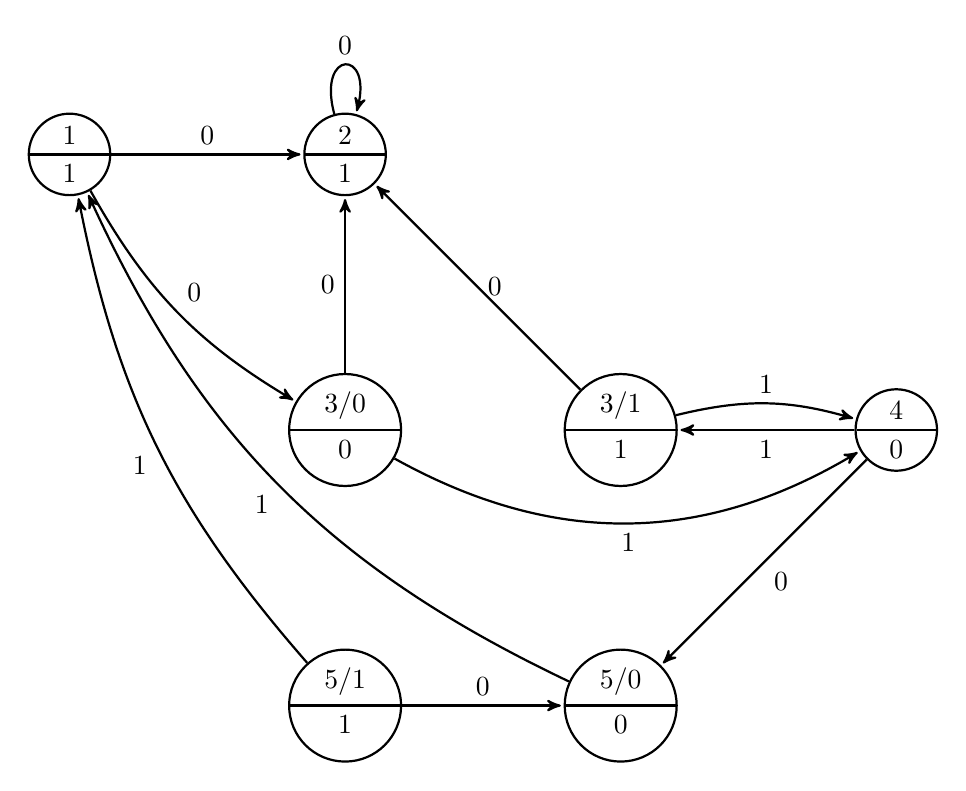
\begin{tikzpicture}[>=stealth',shorten >=1pt,auto,node distance=3.5cm]
%Knoten
\node (1) [state with output, thick] {1 \nodepart{lower} 1};
\node (2) [state with output, thick, right of= 1] {2 \nodepart{lower} 1};
\node (3) [state with output, thick, below of= 2] {3/0 \nodepart{lower} 0};
\node (4) [state with output, thick, right of= 3] {3/1 \nodepart{lower} 1};
\node (5) [state with output, thick, right of= 4] {4 \nodepart{lower} 0};
\node (6) [state with output, thick, below of= 4] {5/0 \nodepart{lower} 0};
\node (7) [state with output, thick, left of= 6] {5/1 \nodepart{lower} 1};

%Verbindungen
\path[thick,->]
(1) edge node {0} (2)
(1) edge [bend angle=15, bend right] node {0} (3)

(2) edge [loop above] node {0} (2)

(3) edge node {0} (2)
(3) edge [bend angle=-30, bend left,below] node {1} (5)

(4) edge [right] node {0} (2)
(4) edge [bend angle=15, bend left] node {1} (5)

(5) edge node {1} (4)
(5) edge node {0} (6)

(6) edge [bend angle=20, bend left] node {1} (1)

(7) edge node {0} (6)
(7) edge [bend angle=15, bend left] node {1} (1)

;
\end{tikzpicture}
\end{center}

\clearpage

\section{Aufgabe 2} 

\vspace{1.5cm}

\begin{tabular}{llll}  
	Z & x & Z+ & y \\ \hline	
	0 & 0 & 1 & 1  \\ 
	0 & 1 & 2 & 1 \\ \hline
	1 & 0 & 2 & 1 \\
	1 & 1 & 1 & 0 \\ \hline
	2 & 0 & 2 & 1 \\
	2 & 1 & 0 & 1 \\	 
\end{tabular}

\vspace{1.5cm}


$Z^+_{0}=Z_{2}x \\
Z^+_{1}=Z_{0}\overline{x}$ v $Z_{1}x \\
Z^+_{2}=Z_{0}x$ v $Z_{1}\overline{x}$ v $Z_{2}\overline{x}$



\vspace{1.5cm}

\begin{center}
	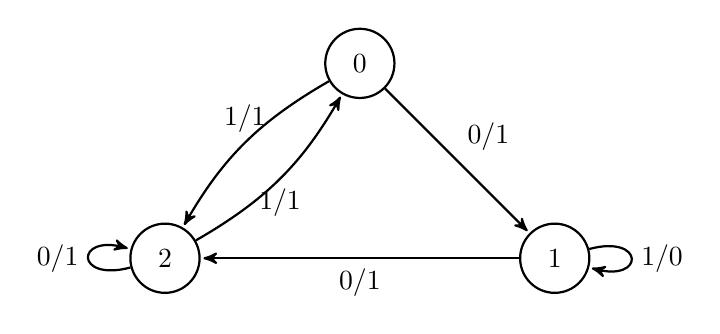
\begin{tikzpicture}[>=stealth',shorten >=1pt,auto,node distance=3.5cm]
	
	%Knoten
	\node (1) [state, thick] {0};
	\node (2) [state, thick, below left of= 1] {2};
	\node (3) [state, thick, below right of= 1] {1};
	
	%Kanten
	\path[thick,->]
	(1)	edge node {0/1} (3)
	(1)	edge [bend angle=15, bend right, above] node {1/1} (2)
	
	(2)	edge [bend angle=15, bend right, below] node {1/1} (1)
	(2)	edge [loop left] node {0/1} (2)
	
	(3)	edge [loop right] node {1/0} (3)
	(3) edge node {0/1} (2);
	
	
	\end{tikzpicture}
\end{center}

\clearpage

\section{Aufgabe 3} 

\vspace{1,5 cm}

\begin{tabular}{cccc}  
	$Z_{1}Z_{0}$& x & $Z^+_{1}Z^+_{0}$ & y \\ \hline	
	00 & 0 & 11 & 0  \\ 
	00 & 1 & 01 & 0 \\ \hline
	01 & 0 & 00 & 1 \\
	01 & 1 & 10 & 0 \\ \hline
	10 & 0 & 11 & 1 \\
	10 & 1 & 01 & 0 \\ \hline
	11 & 0 & 00 & 0 \\
	11 & 1 & 10 & 0 \\
\end{tabular}

\vspace{1,5 cm}

$y=\overline{Z_{1}}Z_{0}x$ v $Z_{1}\overline{Z_{0}}x$ \\
$Z^+_{1}= \overline{Z_{1}}\overline{Z_{0}}\overline{x}$ v x v $Z_{1}Z_0\overline{x}$ \\
$Z^+_{0}=\overline{Z_{1}Z_{0}}x$ v $\overline{Z_{0}}$ v $Z_{1}\overline{Z_{0}x}$

\clearpage

\section{Aufgabe 4} 


\end{document}